\documentclass[11pt]{article}
\usepackage[margin=1in]{geometry}
\usepackage[T1]{fontenc}
\usepackage{lmodern}
\usepackage{amsmath,amssymb,amsthm}
\usepackage{booktabs}
\usepackage{graphicx}
\usepackage{enumitem}
\usepackage[hidelinks]{hyperref}
\setlist{itemsep=2pt,topsep=4pt}

\newtheorem{proposition}{Proposition}
\newtheorem{theorem}{Theorem}
\newtheorem{lemma}{Lemma}
\newtheorem{corollary}{Corollary}

\newcommand{\E}{\mathbb{E}}

\title{Why Governments Do Not Build Funds:\\ Political Turnover, Fund Raiding and the Missing Asset Path\\[4pt] \large Progress report}
\date{4 November 2026}

\begin{document}
\maketitle

\begin{abstract}
\noindent In the planner benchmark of Battaglini and Coate (2008), a government accumulates assets until the interest finances spending and taxes can be zero forever. Real governments, Indian states among them, almost never do this. I study one friction: after a change of government, a successor can divert part of any accumulated fund. Over six model versions this gives (i)~a turnover threshold for saving and three fiscal regimes (borrow, balanced budget, save); (ii)~a precautionary version in which the turnover risk a state can tolerate scales with the \emph{variance} of spending shocks while the cost of raiding is proportional to the raided share; (iii)~a fungibility result, in which legal protection of a sinking fund matters only when borrowing headroom is small; and (iv)~the latest and main result: in an infinite-horizon economy with spending shocks, \emph{any} positive expected raiding removes the planner's long-run anchor. There is no steady state with a finite average marginal cost of public funds. With a debt ceiling, a steady state exists and the ceiling must bind with positive probability, governed by an exact ``wedge accounting'' identity.
\end{abstract}

\section{Question and motivation}

\textbf{Benchmark.} With $\beta(1+r)=1$ and spending uncertainty, the planner in Battaglini and Coate (2008) (see also Aiyagari, Marcet, Sargent and Sepp\"al\"a 2002) front-loads taxes and builds up assets until the interest covers spending; taxes are then zero forever.

\textbf{Puzzle.} Most governments carry debt (Indian general government debt is about 80\% of GDP). Large public funds are rare: Norway, Gulf states, Chile.

\textbf{Question.} Why don't governments accumulate assets as the benchmark prescribes, and which institutions allow some to do so?

\textbf{Mechanism.} The incumbent stays in office with probability $q$. After turnover, the successor diverts a share $\varphi$ of any accumulated assets ($\varphi$ measures how well the fund is protected). The incumbent's effective return on saving is $(1+r)\,[\,q+(1-q)(1-\varphi)\,]$.

\textbf{Setting: Indian states.} Indian states combine high debt, small Consolidated Sinking Funds (CSF) at the RBI, strong anti-incumbency, a return to the Old Pension Scheme in several states (liabilities pushed onto successors), and a net borrowing ceiling set by the Centre.

\textbf{Closest literature.}
\begin{itemize}
\item \emph{Battaglini and Coate (2008)}, the main overlap. Pork for minimum winning coalitions keeps debt above the planner's level. Their friction is \emph{within-period}: part of extra revenue goes to pork whoever governs. Mine is \emph{between-period}: the stock of assets is lost only on turnover. A government sure to stay in office saves at the planner's level here.
\item \emph{Alesina and Tabellini (1990)}: alternating parties that disagree over spending over-borrow. I use their disagreement channel in Version~2.
\item \emph{Battaglini (2014)}: dynamic probabilistic voting with debt as the state; a template for making $q$ endogenous.
\item \emph{Battaglini (2026)}: alternation with a durable state can produce cycles and chaos in Markov equilibrium. This is relevant to my Version~3 numerics.
\end{itemize}

\section{Common environment}

Households have quasi-linear preferences $u=c+A\,v(g)-h(l)$. With a linear labour tax $\tau$ and wage 1, labour supply is $l(\tau)=(1-\tau)^{\varepsilon}$, revenue is $R(\tau)=\tau(1-\tau)^{\varepsilon}$ (Laffer peak at $\tau_p=1/(1+\varepsilon)$), and household surplus is $U(\tau)=(1-\tau)^{1+\varepsilon}/(1+\varepsilon)$. The marginal cost of public funds (MCPF) is
\[
\lambda(\tau)=\frac{-U'(\tau)}{R'(\tau)}=\frac{1-\tau}{1-(1+\varepsilon)\tau},
\]
which rises with $\tau$; this is the reason to smooth taxes. The budget is $g_t+(1+r)b_t=R(\tau_t)+b_{t+1}$, with $b<0$ meaning assets. After turnover, assets are cut by the raid map
\[
T(b)=\begin{cases}(1-\varphi)\,b & b<0\\ b & b\ge 0\end{cases}
\]
so debt is never raided.

\section{Version 1: a two-period threshold}

\textbf{Set-up.} Two periods; spending fixed at $G$; zero initial debt; a benevolent period-1 government saves $a\ge 0$. Budgets: $R(\tau_1)=G+a$; in period~2, $R(\tau_2)=G-(1+r)a$ if the incumbent stays, and $G-(1-\varphi)(1+r)a$ if not.

\textbf{Derivation.} Maximise $U(\tau_1)+\beta[\,qU(\tau_2^S)+(1-q)U(\tau_2^L)\,]$. Using $d\tau/dx=1/R'(\tau)$, the first-order condition is
\[
\lambda(\tau_1)=\beta(1+r)\big[\,q\,\lambda(\tau_2^{S})+(1-q)(1-\varphi)\,\lambda(\tau_2^{L})\big].
\]
At $a=0$ all tax rates are equal, so $\lambda$ cancels. The first rupee is saved iff $\beta(1+r)[1-(1-q)\varphi]>1$, that is,
\[
(1-q)\,\varphi<\kappa\equiv 1-\frac{1}{\beta(1+r)} .
\]
Borrowing at $a=0$ costs $\beta(1+r)\lambda>\lambda$ when $\kappa>0$, so it never happens.

\textbf{Result.} Expected raiding $(1-q)\varphi$ is compared with the patience gap $\kappa$. With $\beta=0.96$ and $r=5\%$, $\kappa\approx0.8\%$, so even small raiding risk stops saving. $\varepsilon$ does not enter the threshold. Above the threshold the budget is balanced: Version~1 explains the absence of assets, but not debt.

\section{Version 2: a disagreeing successor and three regimes}

\textbf{Set-up.} Parties $L$ and $R$ each value only their own public good and both dislike tax distortions; $g$ is chosen with $A v'(g)=\lambda(\tau)$. $L$ governs in period~1. When the period-2 government must repay one more rupee, it raises a share $s$ through taxes and cuts its own good by $1-s$. From the first-order conditions,
\[
s=\Big[1+\frac{\lambda'(\tau)}{-A\,v''(g)\,R'(\tau)}\Big]^{-1}.
\]
Let $d=1-s$: the share of a debt burden that lands on spending $L$ does not value (disagreement).

\textbf{Derivation.} At $b=0$, if $L$ borrows a rupee, under $R$ it bears only the tax part $s$. So borrowing pays iff $\beta(1+r)[q+(1-q)s]<1$, i.e.\ $(1-q)d>\kappa$. If $L$ saves a rupee, under $R$ a share $\varphi$ is raided first and $R$ uses only $s$ of the rest to cut taxes. So saving pays iff $\beta(1+r)[q+(1-q)(1-\varphi)s]>1$, i.e.\ $(1-q)[d+\varphi(1-d)]<\kappa$.

\begin{center}
\begin{tabular}{lll}
\toprule
Regime & Condition at $b=0$ & Example\\
\midrule
Borrow & $(1-q)\,d>\kappa$ & Indian states\\
Balanced budget & in between & \\
Save & $(1-q)\,[d+\varphi(1-d)]<\kappa$ & Norway\\
\bottomrule
\end{tabular}
\end{center}

\textbf{Results.} Turnover and disagreement create debt. Raiding blocks assets but cannot create debt on its own, and the balanced-budget band exists only because $\varphi>0$. With $\kappa=0$ any $q<1$ gives debt, the pure Alesina--Tabellini case. With $v=\log$, $d\approx0.014,\,0.028,\,0.058$ for $\varepsilon=0.25,\,0.5,\,1$. A grid search matched the predicted regime in all 17 cases tried.

\section{Version 3: infinite horizon, and why the benchmark had to change}

\textbf{Set-up.} The state is debt $b$. With symmetric parties, $V$ (party in power) and $W$ (party out of power) satisfy
\[
V(b)=\max_{\tau,g,b'}\;U(\tau)+A\,v(g)+\beta\big[q\,V(b')+(1-q)\,W(T(b'))\big],
\]
\[
W(b)=U(\tau^*(b))+\beta\big[q\,W(b^*(b))+(1-q)\,V(T(b^*(b)))\big],
\]
and I look for a Markov-perfect equilibrium. I solved it by value-function iteration.

\textbf{Findings.} With $\beta(1+r)>1$ and $\varphi>0$, long-run debt is exactly zero, so the balanced-budget band survives. With $\beta(1+r)=1$ and $\varphi=0$, the outcome is Barro ($q=1$) or Alesina--Tabellini debt ($q<1$). Some cases cycled. With $\beta(1+r)>1$ and $q=1$, the planner saved without limit.

\textbf{Consequences.} (1)~The ``save until taxes are zero, then stop'' planner needs $\beta(1+r)=1$ \emph{plus} spending shocks, so Versions~4 and~6 switch to that benchmark. (2)~Following Battaglini (2026), the cycling may reflect complex equilibrium dynamics rather than numerical error.

\section{Version 4: spending shocks with $\beta(1+r)=1$}

\textbf{Set-up.} Version~1 with $\beta(1+r)=1$. Period-2 spending is $G_2=\bar G\pm\sigma$ with equal probability. Let $\Lambda(G)=\lambda(\tau(G))$ be the MCPF at the tax rate that raises $G$, and define the buffer premium $P=\E\Lambda(G_2)/\Lambda(\bar G)-1$.

\textbf{Derivation.} At $a=0$, saving the first rupee gains $[1-(1-q)\varphi]\,\E\Lambda(G_2)$ and costs $\Lambda(\bar G)$, so the government saves iff
\[
(1-q)\varphi<\frac{P}{1+P}\quad\Longleftrightarrow\quad q>q^*=1-\frac{P}{(1+P)\varphi}.
\]

\begin{lemma}[$\Lambda$ is convex]
$\lambda'=\varepsilon/(1-(1+\varepsilon)\tau)^2>0$ and $\lambda''=2\varepsilon(1+\varepsilon)/(1-(1+\varepsilon)\tau)^3>0$. Below the peak, $R'>0$ and $R''=\varepsilon(1-\tau)^{\varepsilon-2}[(1+\varepsilon)\tau-2]<0$. Since $\Lambda'=\lambda'/R'$, we get $\Lambda''=(\lambda''R'-\lambda'R'')/R'^3>0$. Hence $P>0$.
\end{lemma}

\begin{proposition}[More risk, more tolerance]
Any mean-preserving spread of $G_2$ raises $\E\Lambda(G_2)$ (Rothschild--Stiglitz), so it raises $P$ and lowers $q^*$. The turnover risk a state can tolerate and still save rises with spending risk. (This corrects the sign as I stated it in my 11 October email.)
\end{proposition}

\begin{proposition}[Raiding is first order, the buffer second order]
$P=\tfrac12\frac{\Lambda''(\bar G)}{\Lambda(\bar G)}\sigma^2+O(\sigma^4)$. Expanding at small tax rates gives $\Lambda(G)=1+\varepsilon G+\varepsilon(1+2\varepsilon)G^2+O(G^3)$. To leading order,
\[
1-q^*\;\approx\;\frac{\varepsilon(1+2\varepsilon)\,\sigma^2}{\varphi}.
\]
\end{proposition}
The benefit of a buffer scales with the variance of shocks, while the cost of raiding is proportional to $\varphi$. This is why small raiding risks dominate, and it also shows that a higher $\varepsilon$ means more saving. The numerical curvature at $G\to0$ is 0.753, 2.012 and 6.054 against the formula's 0.75, 2 and 6.

\begin{center}
\begin{tabular}{cccc}
\toprule
& \multicolumn{3}{c}{Threshold $q^*$ ($\bar G=0.1$, $\varphi=0.5$)}\\
\cmidrule(l){2-4}
$\varepsilon$ & $\sigma=0$ & $\sigma=0.02$ & $\sigma=0.04$\\
\midrule
0.25 & 1.000 & 1.000 & 0.998\\
0.5 & 1.000 & 0.998 & 0.993\\
1.0 & 1.000 & 0.992 & 0.969\\
\bottomrule
\end{tabular}
\end{center}

\section{Version 5: fungibility of a protected sinking fund}

\textbf{Set-up.} Three periods, $\beta(1+r)=1$. In period~1 the incumbent puts $F\ge0$ into a fund that can only retire debt. In period~2 (election and shock $\bar G\pm\sigma$), a successor cannot touch $F$ but borrows and diverts $x=\varphi\min\{F(1+r),\bar D\}$, where $\bar D$ is the borrowing headroom; the fund repays this in period~3. With $\bar D=\infty$ this is Version~4.

\textbf{Predictions.} (1)~No ceiling: protection is useless. (2)~$\bar D=0$: planner-level saving. (3)~Protection and a ceiling are complements. (4)~The objective has a convex kink at $F(1+r)=\bar D$, so the choice is all-or-nothing. (5)~A ceiling on \emph{net} debt would restore full fungibility.

\textbf{Numerical check} ($\varepsilon=0.5$, $\bar G=0.1$, $\sigma=0.04$, $\varphi=0.5$). The all-or-nothing jump is confirmed: with $\bar D=0.0001$, $F^*=0.00073$ at $q=0.995$ and $F^*=0$ at $q=0.99$. It holds only when $\bar D$ is below the planner's buffer (0.7--5\% of $\bar G$), because the gain from a buffer is second order while the expected raid is first order in $\bar D$.

\textbf{Mapping to Indian rules.} The CSF is held by the RBI, can only redeem liabilities, and withdrawals are capped (terms vary by state and were relaxed in 2020--21). Borrowing is capped by the net borrowing ceiling (about 3\% of GSDP a year) and state FRBM Acts, but nothing links the cap to the fund. India ring-fences the fund but does not link borrowing to it. \emph{Open question:} the ceiling limits gross borrowing minus repayments, so redemptions paid from the CSF may free borrowing room rupee for rupee. If so, the withdrawal rule is the effective $\varphi$.

\section{Version 6 (latest): the long run with raiding}

\subsection{Environment}
\begin{itemize}
\item Infinite horizon, $\beta(1+r)=1$, spending needs $G_t$ i.i.d.\ and non-degenerate.
\item Revenue is $x_t=G_t+(1+r)b_t-b_{t+1}$; if $x_t<0$ the government pays lump-sum transfers valued one-for-one (as in Battaglini--Coate). So $\lambda\ge1$, with $\lambda=1$ at zero taxes.
\item Turnover with probability $1-q$, after which assets become $T(b)$.
\item \emph{Assumption:} every government maximises citizens' welfare, and raided resources are dissipated.
\item Debt is bounded by the natural limit $\bar b_N=(R_{\max}-G_H)/r$, or by a ceiling $\bar D<\bar b_N$ when stated.
\end{itemize}

\begin{proposition}[The equilibrium is a planner problem with a stochastic levy]\label{prop:planner}
The Markov equilibrium solves
\[
V(b,G)=\max_{b'}\;\tilde U\big(G+(1+r)b-b'\big)+\beta\,\E_{G'}\big[q\,V(b',G')+(1-q)\,V(T(b'),G')\big].
\]
$V$ is concave and decreasing in $b$, falls with $1-q$ and with $\varphi$, and cannot be raised by a debt ceiling.
\end{proposition}
\noindent\emph{Proof outline.} An equilibrium value is a fixed point of the Bellman operator, which is a contraction, so it is unique. $T$ is convex, and a concave decreasing function of a convex map is concave, so the operator preserves concavity. Monotonicity in $(q,\varphi)$ follows because $V(T(b'))\le V(b')$ and $T$ rises with $\varphi$. A ceiling only shrinks a single optimiser's choice set.

\begin{lemma}[Euler conditions and the wedge]\label{lem:wedge}
Let $\omega_t=\E_t\lambda_{t+1}-\lambda_t$, where $\lambda_{t+1}$ is next period's realised MCPF. Comparing the gain from borrowing one more rupee today ($\lambda_t$) with its expected cost tomorrow:
\begin{center}
\begin{tabular}{lll}
\toprule
Choice of $b'$ & Optimality & Wedge $\omega_t$\\
\midrule
Fund, $b'<0$ & $\lambda_t=\E_t[q\lambda^S+(1-q)(1-\varphi)\lambda^R]$ & $(1-q)\varphi\,\E_t\lambda^R\ \ge (1-q)\varphi>0$\\
Zero debt & $(1-(1-q)\varphi)\E_t\lambda_{t+1}\le\lambda_t\le\E_t\lambda_{t+1}$ & $\ge 0$\\
Debt, $0<b'<\bar D$ & $\lambda_t=\E_t\lambda_{t+1}$ & $0$\\
At the ceiling & $\lambda_t\ge\E_t\lambda_{t+1}$ & $\le 0$\\
\bottomrule
\end{tabular}
\end{center}
\end{lemma}
\noindent The first row is the key one. The government weights the raided outcome by $1-\varphi$ because the money is gone, but that high-cost outcome still happens in full. Without a ceiling, the MCPF is therefore a \emph{submartingale}. For the planner it is a martingale bounded below by~1, so it converges to~1, which is the zero-tax fund.

\begin{theorem}[Raiding removes the fiscal anchor]\label{thm:anchor}
If $q<1$, $\varphi>0$ and there is no ceiling below the natural limit, there is no stationary distribution of $(b,G)$ with $\E\lambda<\infty$. In particular, the planner's zero-tax fund is never a steady state, for any $(1-q)\varphi>0$.
\end{theorem}
\noindent\emph{Proof outline (by contradiction).}
\begin{enumerate}
\item \emph{Zero drift.} In a stationary distribution, $\E\lambda_{t+1}=\E\lambda_t$, so $\E\omega_t=0$. Since $\omega_t\ge0$, $\omega_t=0$ almost surely. So no fund is held (there $\omega_t>0$), and $\lambda$ is a martingale.
\item \emph{Frozen MCPF.} A martingale bounded below converges almost surely (Doob), so $\lambda_{t+1}-\lambda_t\to0$. Under stationarity this difference has the same law in every period, so $\lambda_{t+1}=\lambda_t$ almost surely: the tax rate never changes.
\item \emph{Contradiction.} With constant revenue $\bar x$, $b_{t+1}=(1+r)b_t+G_t-\bar x$, and $\operatorname{Var}(b_t\mid\mathcal F_0)=\operatorname{Var}(G)\sum_{s<t}(1+r)^{2s}\to\infty$. (With $\lambda\equiv1$ and no fund, debt grows by at least $G_L$ each period.) Debt cannot stay bounded.
\end{enumerate}
For the planner, step~3 fails at the zero-tax fund, because transfers vary and absorb the shocks. With raiding, reaching that point requires holding a fund, which is exactly where the MCPF is pushed up. The argument is the martingale method of Chamberlain and Wilson (2000), applied here to raided public funds.

\begin{theorem}[The debt ceiling as anchor]
With a ceiling $\bar D<\bar b_N$:
\begin{enumerate}[label=(\alph*)]
\item a stationary distribution $\mu$ exists;
\item \emph{wedge accounting}: $\;\E_\mu[\,|\omega|\,;\text{ceiling binds}\,]=(1-q)\varphi\,\E_\mu[\lambda^R;\,b'<0]+\E_\mu[\omega;\,b'=0]$;
\item if $q<1$ and $\varphi>0$, the ceiling binds with positive probability; for the planner the probability goes to~0;
\item $P_\mu(\text{fund held})\le \E_\mu[\,|\omega|\,;\text{ceiling binds}\,]\,/\,[(1-q)\varphi]$.
\end{enumerate}
\end{theorem}
\noindent\emph{Proof outline.} (a)~The state space is compact and the policy is continuous, so Krylov--Bogolyubov applies. (b)~$\E_\mu\omega=0$; split by the rows of Lemma~\ref{lem:wedge} (the interior contributes~0). (c)~If the ceiling never bound, steps 1--3 above would apply on a bounded state space. (d)~Follows from (b), using $\lambda^R\ge1$ and that the zero-debt term is non-negative.

\textbf{Reading.} On average, the ceiling absorbs exactly the upward pressure that raiding and inaction create. Holding a fund a share $p$ of the time requires a ceiling that bites at least $p(1-q)\varphi$ on average, so protection and ceilings are complements (the dynamic version of Version~5).

\subsection{Numerical verification}
The model is solved by time iteration on the Euler equations with endogenous grid points, which handles the kink at zero debt exactly. Parameters: $\varepsilon=0.5$, $r=5\%$, $G\in\{0.06,0.14\}$. The natural limit is 4.90, and the zero-tax fund is 2.80 (28 years of average spending).

\begin{figure}[h]
\centering
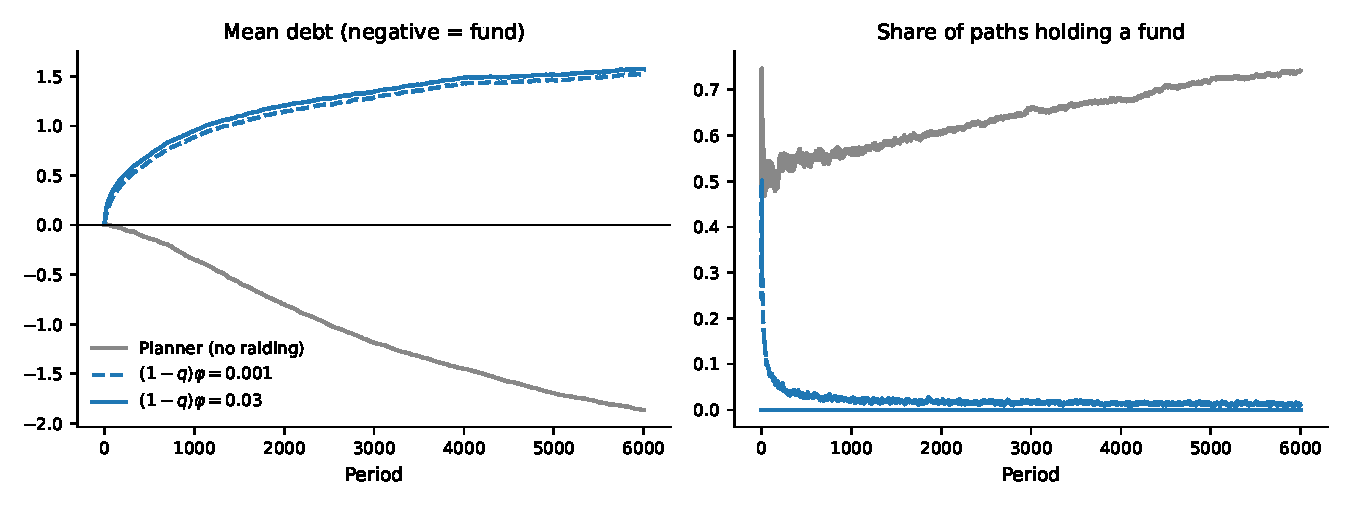
\includegraphics[width=\textwidth]{fig_v6_longrun.pdf}
\caption{No ceiling, 3{,}000 paths from zero debt. The planner moves toward the zero-tax fund. With raiding, funds disappear and mean debt rises. An expected loss of 0.1\% a year behaves almost like 3\%.}
\end{figure}

\begin{center}
\small
\begin{tabular}{lcccccc}
\toprule
Case (with ceiling $\bar D$) & Binds & Zero debt & Fund & Raid + inaction & Ceiling & Bound (d)\\
& & & & wedge & wedge & \\
\midrule
$q=0.9,\ \varphi=0.3,\ \bar D=1.0$ & 0.28\% & 0.47\% & 0 & 0.000044 & 0.000044 & $0\le0.0015$\\
$q=0.9,\ \varphi=0.3,\ \bar D=0.5$ & 0.86\% & 1.21\% & 0 & 0.000113 & 0.000113 & $0\le0.0038$\\
$q=0.9,\ \varphi=0.3,\ \bar D=0.25$ & 2.75\% & 3.54\% & 0 & 0.000343 & 0.000342 & $0\le0.0114$\\
$q=0.99,\ \varphi=0.1,\ \bar D=0.5$ & 0.70\% & 0 & 8.75\% & 0.000091 & 0.000092 & $0.0875\le0.0917$\\
Planner, $\bar D=0.5$ & $\to0$ & 0 & 95\% & 0 & $\approx0$ & --\\
\bottomrule
\end{tabular}
\end{center}
The distributions are stationary (averages over periods 3{,}000--6{,}000), and the identity holds to six decimals.

\subsection{Limits}
\begin{enumerate}
\item The $\beta(1+r)=1$ benchmark: with $\beta(1+r)<1$ the planner does not build a fund either.
\item Dissipated raids: if parties valued their own raids, strategic terms would appear and Proposition~\ref{prop:planner} would no longer hold.
\item $q$ and $\varphi$ are reduced forms.
\item Theorem~\ref{thm:anchor} gives no speed of drift (in simulations debt spreads slowly, like a reflected random walk).
\end{enumerate}

\section{Questions for discussion}
\begin{enumerate}
\item Is the $\beta(1+r)=1$ benchmark with dissipated raids an acceptable main setting, keeping Versions~1--2 as simple illustrations?
\item Is applying the Chamberlain--Wilson argument to raided public funds a contribution worth building the paper around?
\item Next step: add Alesina--Tabellini disagreement to Version~6 (a debt-region wedge, which should make the ceiling bind more often), or make $q$ endogenous via probabilistic voting (Lindbeck and Weibull 1987; Battaglini 2014)?
\item Is the prediction that borrowing ceilings must bind regularly worth taking to Indian state data (utilisation of the net borrowing ceiling, CSF balances)?
\end{enumerate}

\section*{References}
\small
\begin{itemize}[label={},leftmargin=0pt]
\item Aiyagari, R., A. Marcet, T. Sargent and J. Sepp\"al\"a (2002), \emph{Journal of Political Economy}.
\item Alesina, A. and G. Tabellini (1990), \emph{Review of Economic Studies}.
\item Battaglini, M. (2014), ``A dynamic theory of electoral competition'', \emph{Theoretical Economics} 9: 515--554.
\item Battaglini, M. (2026), ``Chaos and unpredictability with time inconsistent policy makers'', \emph{Theoretical Economics} 21: 241--280.
\item Battaglini, M. and S. Coate (2008), \emph{American Economic Review}.
\item Chamberlain, G. and C. Wilson (2000), \emph{Review of Economic Dynamics}.
\item Khemani, S. (2004), \emph{Journal of Development Economics}.
\item Lindbeck, A. and J. Weibull (1987), \emph{Public Choice}.
\item Rothschild, M. and J. Stiglitz (1970), \emph{Journal of Economic Theory}.
\end{itemize}

\vspace{6pt}
\noindent\emph{Note:} derivations were checked, and the numerical code written, with the help of an AI assistant (Claude, Anthropic). Code and full proofs are available on request.

\end{document}
